\documentclass{a0poster}

\usepackage{fancytikzposter}
\usepackage{tikz}
\usepackage{xcolor}
\usepackage{titlesec}
\usepackage{array}
\usepackage[slovak]{babel}
\usepackage[utf8]{inputenc}
\usepackage[IL2]{fontenc}
\usepackage[utf8]{inputenc}
\usepackage{wrapfig}
\usepackage{xspace}
\usepackage{graphicx}
\usepackage{multirow}
\usepackage{scalefnt}
\usepackage{adjustbox}
\usetikzlibrary{positioning, shapes, trees, graphs} % RNA trees

\usetemplate{1}
\setblockspacing{0.5}
\setblocktitleheight{1}
\setmargin{3}

\newcommand{\odkaz}[2]{\href{#1#2}{\nolinkurl{#2}}}
\def\Autor{Richard Eliáš}
\def\AutorDH{\textmd{vedúci práce} David Hoksza}
\def\email{\odkaz{mailto:}{richard.elias@matfyz.cz}}
\def\Fakulta{Matematicko-fyzikální fakulta}
\def\Nazov{Vizualizace sekundární struktury RNA s využitím existujících struktur}

\newcommand{\scale}{} %iba aby som mohol pouzivat vsade renewcommand
\newcommand{\height}{} %dtto
\newcommand{\mc}[1]{\multicolumn{1}{c}{#1}}
\newcommand{\ted}[0]{\textit{tree-edit-distance}\hspace{5pt}}
\renewcommand{\O}[1]{\sloppy\mbox{\ensuremath{\mathcal{O}}(#1)}}
\renewcommand{\baselinestretch}{1.3} %riadkovanie
\newcommand{\addfigure}[1]{\begin{tikzpicture}[every node/.style = {rectangle, fill = none, draw = none}]#1\end{tikzpicture}}
\newcommand{\newcolumn}[1]{\addfigure{\node{#1};}} % vkladanie stlpcov obsahujucich obrazky do tabulky

\usepackage[pdftex,unicode]{hyperref} % Musí být za všemi ostatními balíčky
\hypersetup{pdftitle={\Nazov}}
\hypersetup{pdfauthor={\Autor}}


\renewcommand{\BackgroundPicture}{} %biele pozadie



\title{\scalebox{2.}{\Nazov}}
\author{\Autor, \AutorDH\\\Fakulta\\\texttt{\email}}
\begin{document}

\AddToShipoutPicture{\BackgroundPicture}
\noindent
\begin{tikzpicture}
  \initializesizeandshifts
  \titleblock{65}{1}
  \blocknode{Motivácia a ciele práce}{
    Molekula RNA sa stáva predmetom mnohých štúdií, vďaka čomu rastie
    dopyt po nástrojoch pomáhajúcich pri jej analýze. Vlastnosti molekuly
    sú síce ovplyvnené primárou štruktúrou (poradím nukleotidov v~reťazci),
    no viac závisia na ich priestorovom usporiadaní (terciárna štruktára).
    My sa v~práci zaoberáme trochu zjednodušeným modelom - sekundárnou
    štruktúrou. Tú reprezentuje zoznam nukleotidov spojených väzbou.
    Tieto nukleotidy musia byť blízko aj v~priestore a~tak nám sekundárna štruktúra
    relatívne dobre aproximuje terciárnu, pre ktorú neexistujú spoľahlivé
    metódy zisťovania štruktúry už ani pre relatívne malé molekuly.

    Prvým krokom pri analýze RNA molekuly je často rozbor obrázka jej sekundárnej
    štruktúry. Medzi základné kritéria ktoré musia obrázky molekúl spľňať
    patrí rovinnosť nakreslenia, kreslenie loopov na kružnice a~stemy na priamkách.
    Pri porovnávaní štruktúr sa využíva taktiež kreslenie častí majúcich podobnú
    funkciu a~tvar na rovnaké miesta v~obrázkoch, čo pomáha lepšej orientácií
    v~molekule a~napomáha nájsť konzervované časti v~molekulách.
    V súčastných nástrojoch (mFold, RNAViz, RNAView, $\cdots$) sa toto posledné
    kritérium nedodržuje, čo má za následok ťažké nachádzanie konzervovaných častí
    v~molekulách.

    Cieľom našej práce je umožniť vizualizovanie molekúl podľa predstáv biológov.
    Tie bude reprezentovať obrázok vzorovej molekuly podľa ktorej sa budeme snažiť
    nakresliť cieľovú.
  }

  \renewcommand{\scale}{0.25\textwidth}
  \blocknode{Kreslenie chýbajúcich častí v molekule}{
    \begin{wrapfigure}{R}{0.27\textwidth}
      \vspace{-2.7cm}
      \addfigure{
        \node {
          %trim=left bottom right top
          \includegraphics[clip, trim = 1cm 25cm 7cm 1cm, width=\scale]{./include/stem}
        };
      }
      \vspace{-3cm}
    \end{wrapfigure}
    Po transformácií šablónovej molekuly na cieľovú, získavame čiastočnú vizualizáciu
    cieľovej RNA a jej zvyšok potrebujeme dopočítať. Po operáciách delete nám v obrázku
    ostávajú prázdne miesta, naopak po insertoch potrebujeme pre dané vrcholy urobiť
    v obrázku miesto.

    \begin{wrapfigure}{L}{0.27\textwidth}
      \vspace{-2cm}
      \addfigure{
        \node {
          %trim=left bottom right top
          \includegraphics[clip, trim = 0cm 17.5cm 5cm 0cm, width=\scale]{./include/multibranch-redraw}
        };
      }
    \end{wrapfigure}

    Mazanie vrcholov stromu je inverzná operácia ku vkladaniu a tak si ukážeme iba vkladnie.
    Vkladanie báz do loopu (okrem multibranch) je jednoduché, vytvoríme si iba novú kružnicu na ktorú všetky
    bázy uložíme. Vkladanie báz do stemu potrebuje najprv urobiť pre nich najprv urobiť
    miesto a tak celú štruktúru posunie smerom od rodičovského vrcholu v strome.
    Algoritmus vkladania je uvedený na obrázku.

    Pre multibranch loopy je to trochu zložitejšie, chceme sa totiž vyhnúť prípadom, kedy ju musíme
    celú prekresliť, keďže pri tom vznikajú veľké problémy s prekryvmi.
    Prekresleniu štruktúry sa nevyhneme, ak sa jedná o vkladanie veľkého počtu báz, alebo
    vkladáme celú novú vetvu RNA.
  }

  \renewcommand{\scale}{0.25\textwidth}
  \newcommand{\id}[2]{#1 {\small \texttt{(#2)}}}
  \blocknode{Príklady vizualizácií: \id{človek}{K03432} a \id{žaba}{X04025}, \id{mušľa}{L24489} a \id{cikáda}{U06478}, \id{žiabronôžka}{X01723} a \id{pásomnička}{U27015}}{
    \begin{tikzfigure}
      \begin{adjustbox}{totalheight=22cm}
        \begin{tabular}{c c c}
          \newcolumn{
            %trim=left bottom right top
            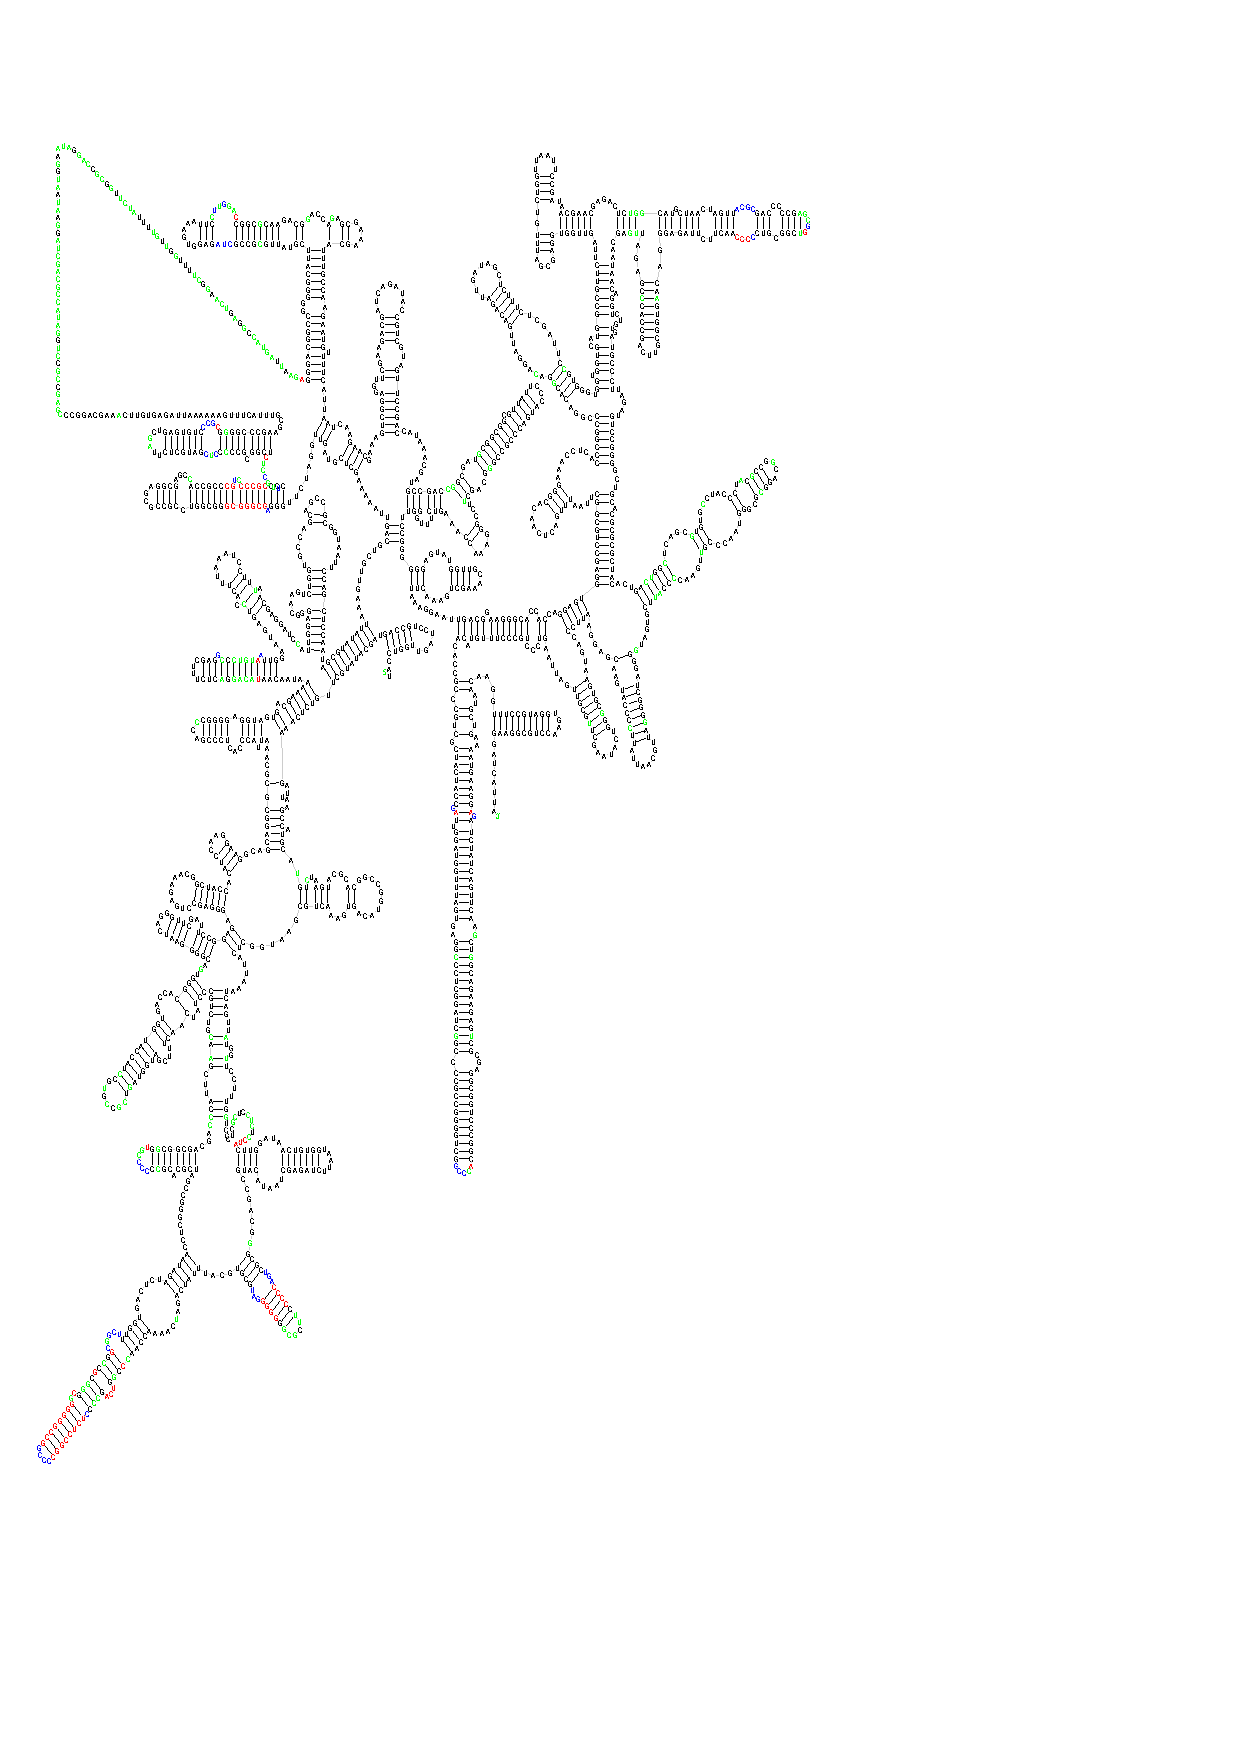
\includegraphics[clip, trim = 0 4cm 7cm 2cm, width=\scale]{./include/human-DRAW-TO-african_frog}
          } & \newcolumn{
            %trim=left bottom right top
            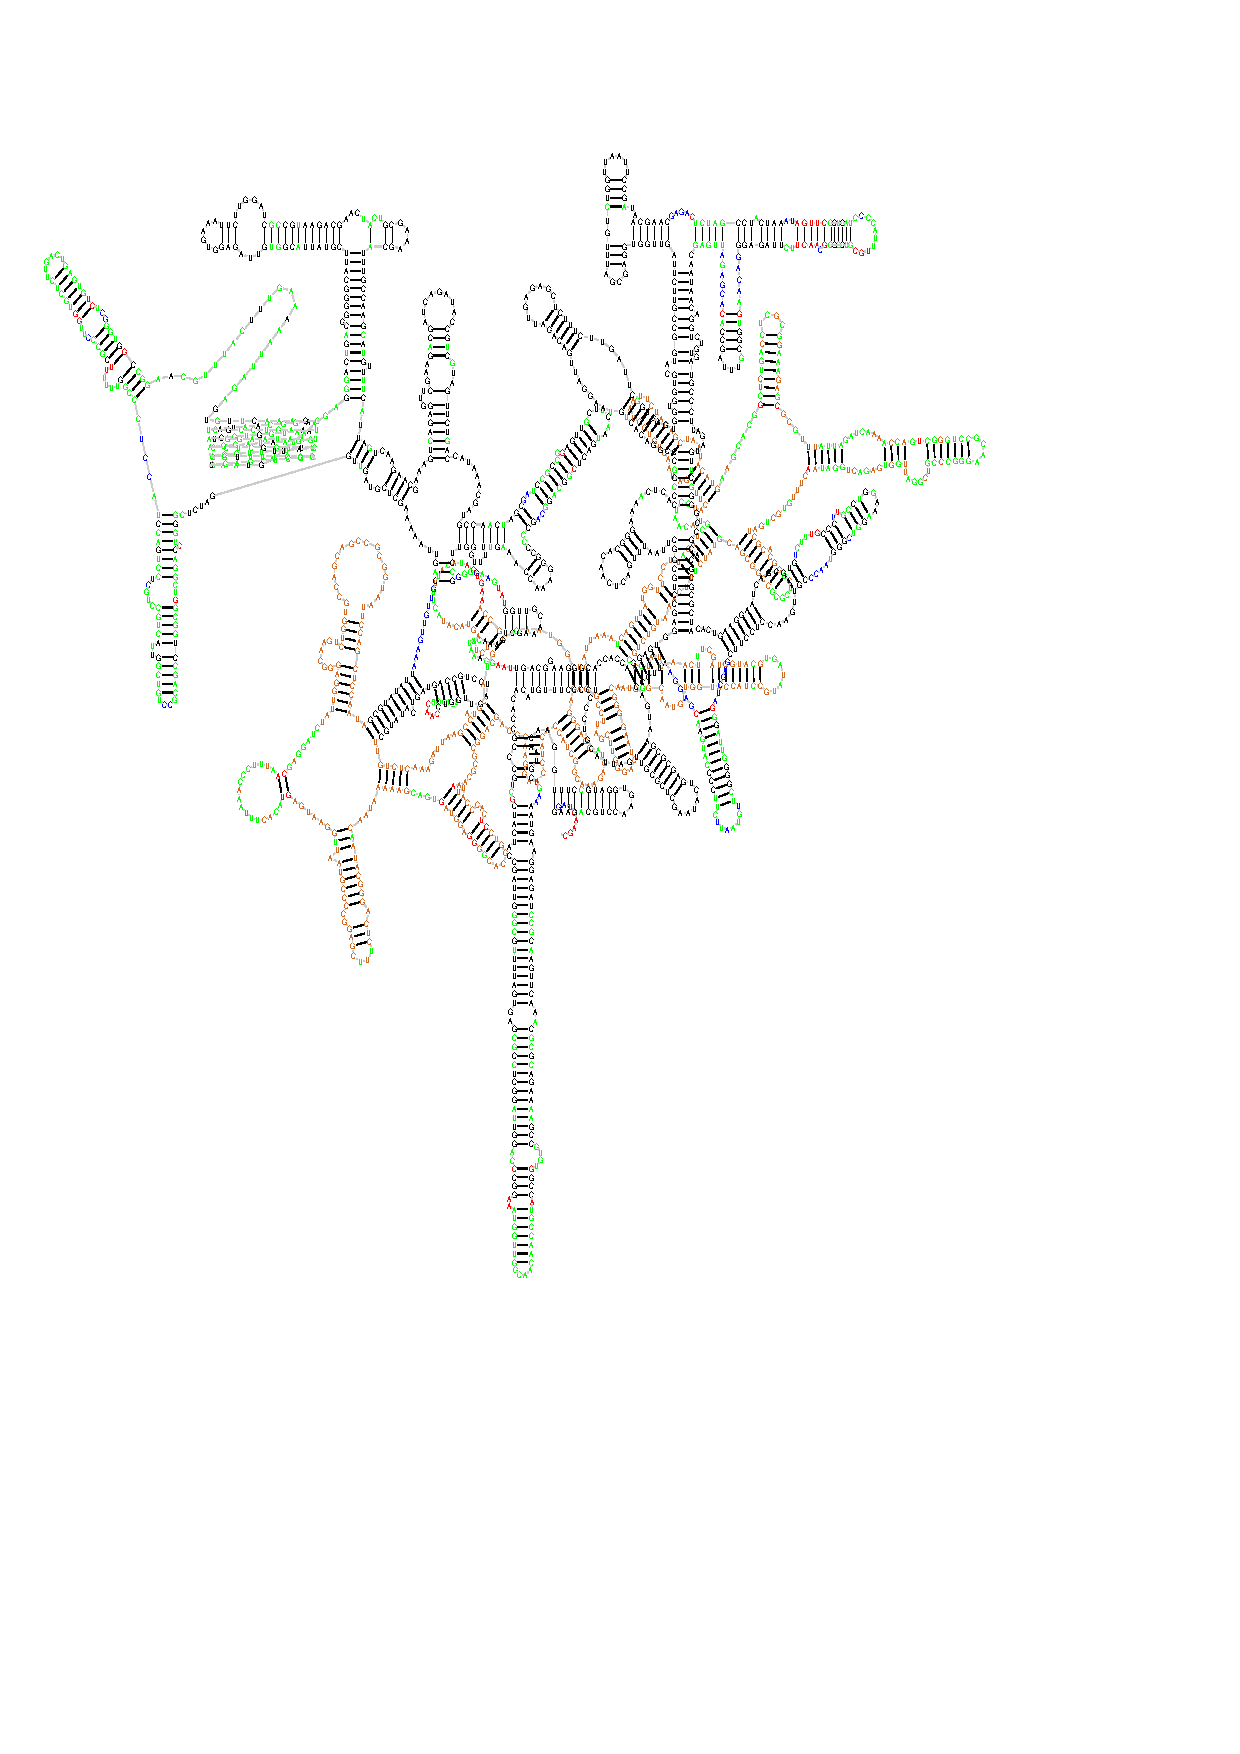
\includegraphics[clip, trim = 0.5cm 4cm 4cm 2cm, width=0.29\textwidth]{./include/blue_mussel-DRAW-TO-cicadas}
          } & \newcolumn{
            %trim=left bottom right top
            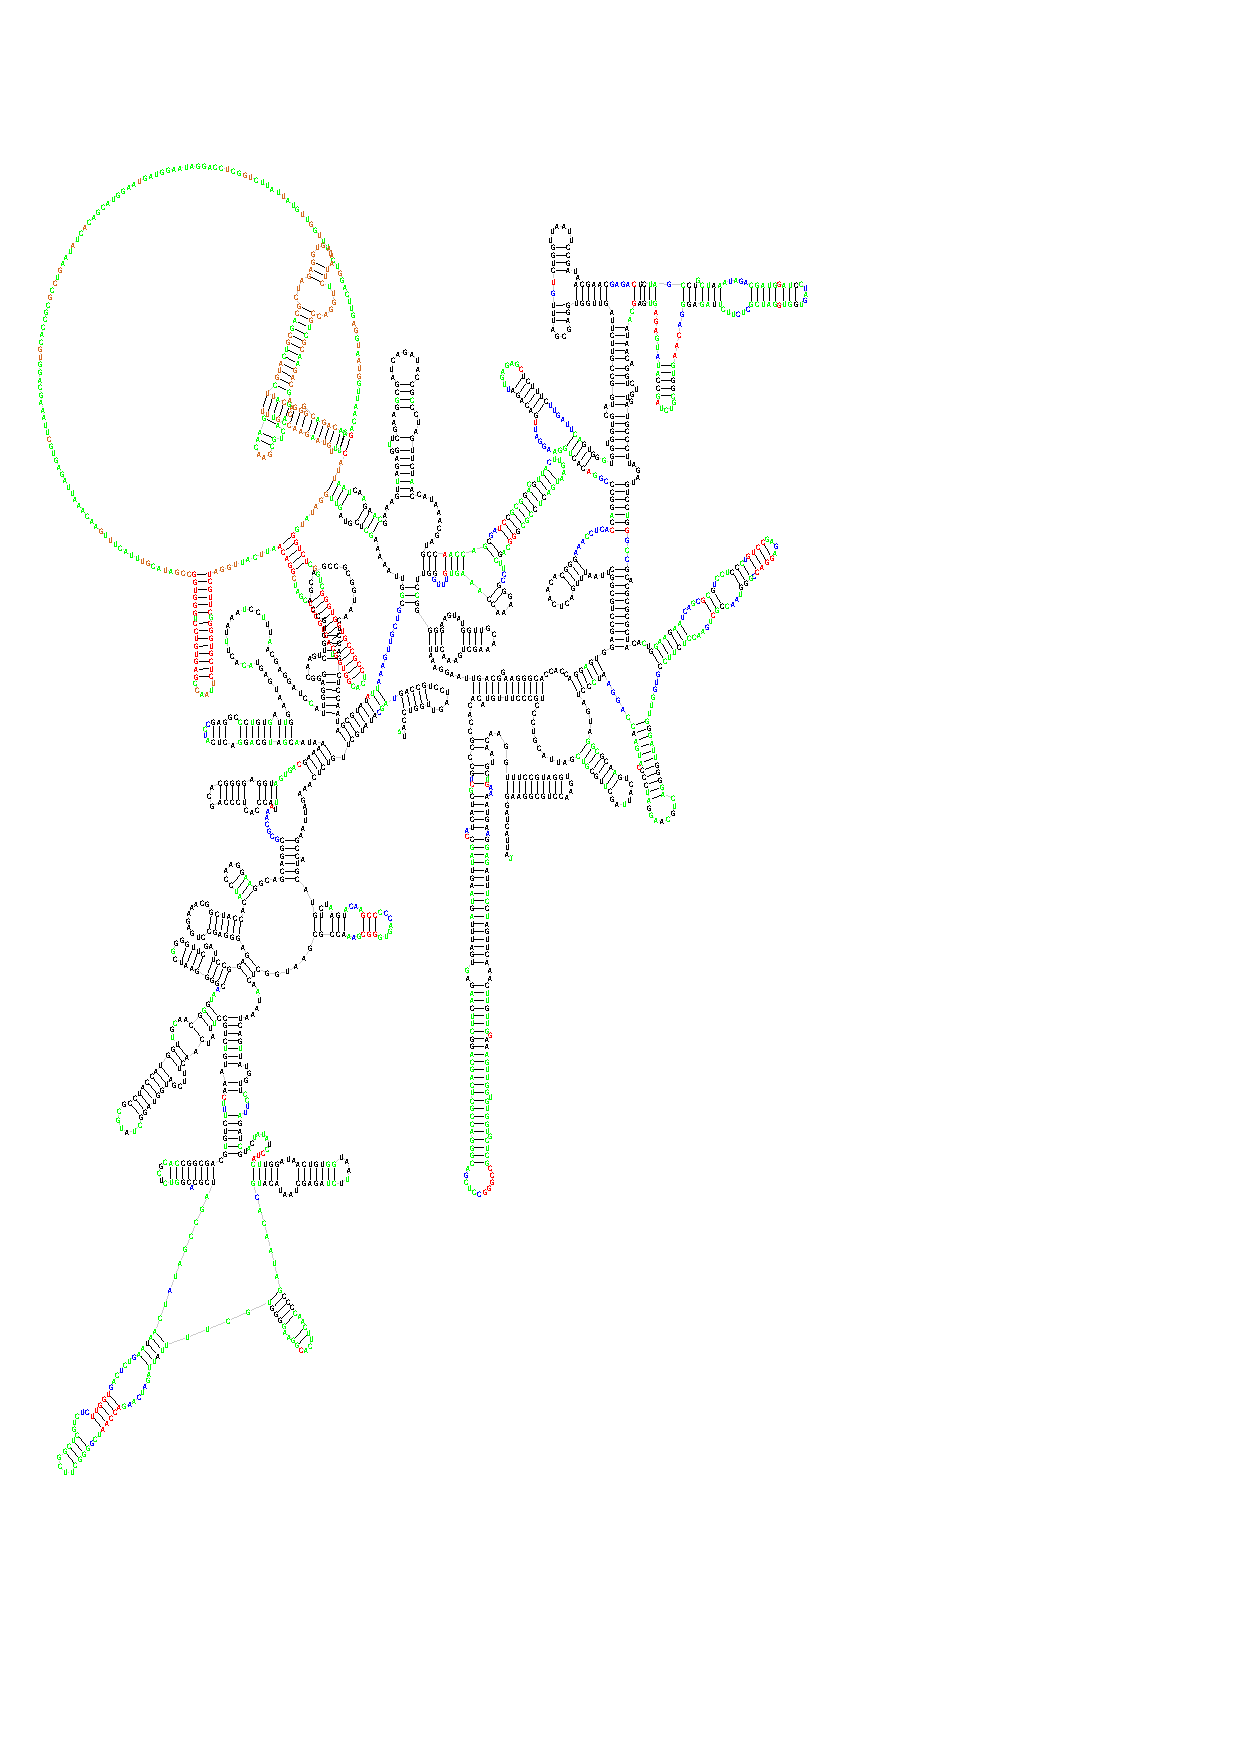
\includegraphics[clip, trim = 0 4cm 7cm 2cm, width=\scale]{./include/artemia_salina-DRAW-TO-echinococcus_granulosus}
          }
        \end{tabular}
      \end{adjustbox}
    \end{tikzfigure}
  }


  %%%%%%%%%%%%%%%%%%%%%%%%%%%%%% DRUHY STLPEC %%%%%%%%%%%%%%%%%%%%%%%%%%%%%%%%%
  \startsecondcolumn

  \blocknode{Stromová reprezentácia RNA a~použitie \ted algoritmu}{
    RNA sekundárnu štruktúru reprezentujeme ako usporiadaný zakorenený strom.
    Vďaka tomu môžeme využiť stromové algoritmy, ako napríklad \ted algoritmus.
    Ten rekurzívnym vzorcom spočíta vzdialenosť medzi stromami a~následne vie
    aj transformovať jeden strom na iný.
    Na príklade ukážeme postup výpočtu a~transformáciu medzi stromami.

    \renewcommand{\scale}{0.25\textwidth}
    \begin{tikzfigure}
      \begin{adjustbox}{totalheight=22cm}
        \begin{tabular}{c c c}
          \\[-3cm]
            \newcolumn{
              %trim=left bottom right top
              \includegraphics[clip, trim = 4cm 12cm 3cm 11cm, width=\scale]{./include/rna_tree}
            } & \newcolumn{
              %trim=left bottom right top
              \includegraphics[clip, trim = 7cm 12.5cm 6cm 11cm, width=\scale]{./include/ted}
            }
            \\[-1cm]
            \newcolumn{
              %trim=left bottom right top
              \includegraphics[clip, trim = 4cm 14cm 11.5cm 13cm, width=\scale]{./include/gted-forest_dist}
            } & \newcolumn{
              %trim=left bottom right top
              \includegraphics[clip, trim = 8cm 12cm 6cm 11cm, width=\scale]{./include/gted-tree_dist}
            } & \newcolumn{
              %trim=left bottom right top
              \includegraphics[clip, trim = 10cm 11.5cm 3.5cm 11cm, width=\scale]{./include/gted-forest_dist}
            }
            \\[-2cm]
        \end{tabular}
      \end{adjustbox}
    \end{tikzfigure}
  }
  \blocknode{Nástroj TRAVeLer}{
    V~rámci práce sme implementovali nástroj TRAVeLer (Template RnA VisuaLization)
    schopný vizualizovať aj veľke rRNA molekuly podľa vstupného vzorového obrázka.
    Implementujeme v~ňom \ted algoritmus, ktorý nám transformuje jednu molekulu na druhú.
    Následným použitím nášho dokresľovacieho algoritmu vznikne výsledná vizualizácia.
    Na príklade ilustrujeme vstupy a výstupy programu. Vstupom sú dve RNA sekundárne štruktúry,
    vzorová potrebuje aj obrázok. Výstupom je obrázok cieľovej molekuly, alebo mapovanie medzi
    štruktúrami (ak si chceme vygenerovať viac typov obrázkov, nemusíme nanovo počítať mapovanie).

    \coloredbox{colorthree!50!}{
      \# ./traveler
        \--\--match-tree mouse.fasta
        \--\--template-tree human.ps human.fasta
        \--\--all mouse\_to\_human
    }

    \vspace{-1cm}
    Aby bolo hľadanie rozdielnych častí jednoduchšie, zaviedli sme farebné kódovanie
    nukleotidov v~obrázku: \textbf{červená} - insert, \textbf{zelená} - edit,
    \textbf{modrá} - prekreslenie báz, \textbf{hnedá} - prekreslenie multibranch loopy.
  }

  \renewcommand{\scale}{0.35\textwidth}
  \blocknode{Výsledky experimentov}{
    \begin{wrapfigure}{L}{\scale}
      \vspace{-1cm}
      \addfigure{
        \node {
          %trim=left bottom right top
          \includegraphics[width=0.33\textwidth]{./include/prekryvy-pocetmolekul}
        };
      }
    \end{wrapfigure}
    Program sme testovali na reálnych obrázkoch 16 molekúl malej podjednotky 18S ribozomálnej RNA
    z~CRW databázy. Z testov sme získali 256 výsledných vizualizácií (každý s~každým).

    Celkové štatistiky prekryvov ukazuje graf. Pre prípady molekúl, ktoré nepotrebovali prekresliť
    multibranch loop sa štatistika zmenila - do 10 prekryvov bolo 150 nakreslení, nad 10 iba 29.

    Počty prekryvov v~závislosti na vzdialenosti TED nieje až taká zjavná. Ak vezmeme najbližšie
    štruktúry, je v~priemere asi 5 prekryvov a~so zväčšujúcou sa vzdialenosťou rástli výkyvy hlavne kvôli tomu,
    že niektoré štruktúry boli dobre konzervované a~na druhej strane bolo pár extrémov, ktoré sa vizualizovali
    veľmi ťažko.

    V~budúcnosti by bolo vhodné upraviť kresliace algoritmy, implementovať otáčanie vetiev RNA stromov v~prípade
    indikovania prekryvov alebo pridať interaktívny nástroj na úpravu obrázkov, čím by užívateľ prekryvy mohol
    ručne odstrániť.
  }
\end{tikzpicture}
\end{document}
